\section{Literature Review}
\label{section:LR}
\subsection{Maritime Semantic Segmentation for USV}
USVs are comprised of several critical modules, including the sensing module, perception module, path planning 
module, and control module \cite{MODS}. Within the perception module, the capacity for environmental perception 
is of paramount importance. Given the physical constraints of small USVs, utilizing cameras as the foundational 
sensing component is a more viable solution \cite{lightsensor1}, \cite{lightsensor2}. In camera-based collision 
avoidance systems for USVs, it is essential to detect both static and dynamic obstacles within the environment. 
Traditional object detection algorithms, however, often fall short in accuracy and provide insufficient 
decision-making information for the path planning module \cite{SSsurvey}. In contrast, semantic segmentation is 
capable of effectively bridging the semantic gap between low-level features and high-level semantics, thereby 
enabling more precise environmental perception.

Another significant challenge in environmental perception for USVs is the complexity of the surrounding 
maritime environment. Many maritime object detection algorithms operate under the assumption that obstacles 
are clearly distinguishable from their background \cite{marineobjdetect1}, \cite{marineobjdetect2}. However, this 
assumption often fails in practice due to factors such as fog, water surface reflections, lens obstructions, 
and the presence of reflections of objects on the water, all of which can make obstacles visually similar 
to the water surface. Background subtraction methods are also prone to errors due to the constant motion of 
the sea \cite{backsub}. By contrast, semantic segmentation algorithms offer a more effective approach to 
extracting relevant information in such scenarios. Given its advantages, algorithms in the USV perception 
module are increasingly inclined to use per-pixel labelled outputs from semantic segmentation as input for 
the path planning module \cite{MODS}, \cite{WaSR}, \cite{MaSTr1325}, \cite{MODD2}.

Although semantic segmentation has been established as the primary task, the vast number of available algorithms 
necessitates careful consideration when selecting the most appropriate one. Based on the level of supervision, 
semantic segmentation methods can be categorized into supervised, semi-supervised, and unsupervised approaches 
\cite{SSsurvey}. Supervised methods, in particular, provide more controllable performance and higher accuracy 
with less training difficulty when high-quality datasets are available \cite{semisupervised}. As a result, most 
maritime semantic segmentation approaches rely on supervised methods. Context-based methods like PSP-Net 
\cite{PSPNet} and DeepLab3+ \cite{Deeplab3+}, as well as feature-enhancement-based methods such as FCN 
\cite{FCN} and U-Net \cite{UNet}, are widely employed in the USV domain for semantic segmentation within 
supervised learning approaches. The following discussion will focus on these CNN architectures and their 
applications in USV domain.

\subsection{CNN Architectures}
We have discussed the context-based methods like PSPNet \cite{PSPNet} and DeepLab3+ \cite{Deeplab3+}, 
which utilize ResNet \cite{resnet} as their backbone, and feature-enhancement-based methods like FCN utilize 
VGG16 \cite{VGG} as its backbone and U-Net \cite{UNet} built upon FCN. While USV and UGV semantic segmentation 
tasks are similar, USV technology lags behind UGV technology \cite{MaSTr1325}. Therefore, applying methods from 
the UGV field can be highly beneficial for USVs. In the UGV domain, deconvolution-based methods, with SegNet 
\cite{SegNet} being a notable architecture, are used for semantic segmentation. This section will discuss the 
potential applications of PSPNet, DeepLab3+, U-Net, and SegNet, as well as their potential in the USV domain.

PSPNet, introduced in 2017 by Zhao et al.\cite{PSPNet}, quickly garnered attention in the field of image 
segmentation. Sun et al.\cite{pspnet-ugv} developed an algorithm based on this architecture for image 
segmentation in autonomous driving under rainy conditions. Besides, Zhu et al.\cite{pspnet-cad} applied PSPNet 
to coronary angiography image segmentation, achieving more accurate results than those obtained with U-Net. 
In the USV domain, Yin et al. \cite{pspnet-shoreline} utilized this architecture to develop a shoreline 
recognition algorithm.

U-Net was introduced in 2015 by Ronneberger et al. \cite{UNet} and has since spawned numerous derivative 
architectures \cite{h-dense-unet,3dunet,unet++}. It is particularly widely used in the field of medical 
image segmentation \cite{SSsurvey}. U-Net has been applied to various image modalities, including Magnetic 
Resonance Imaging (MRI), Computed Tomography (CT), Retinal Fundus Imaging, Microscopy, Dermoscopy, Ultrasound, 
and X-Ray \cite{unet-med-reveiw}.

The DeepLab family leverages atrous convolution to expand the receptive field, allowing it to capture 
multiscale contextual information \cite{Deeplab3+}. Yurtkulu et al. \cite{deeplabv3-ugv} developed an 
extended DeepLabv3 framework tailored for the UGV domain. This precise ability to capture fine details 
has also made DeepLab highly favoured in the medical field, as demonstrated by Azad et al. \cite{deeplabv3+-med}, 
who applied DeepLab3+ for skin lesion detection.

SegNet was initially developed for understanding road and indoor scenes, offering efficiency in memory usage and 
computational time \cite{SegNet}. Over time, it has been applied to tasks such as crack detection \cite{segnet-crack} 
and medical image processing \cite{segnet-med}, demonstrating its versatility. All of these architectures show 
potential for application in the USV domain, or have already been utilized in this context. However, their specific 
performance in USV applications remains largely unexplored. Some researchers have begun comparing the effectiveness 
of these architectures for USV tasks, laying the groundwork for selecting the most suitable option among these four 
major architectures.

In the study of the WaSR algorithm, researchers evaluated the performance of PSPNet, SegNet, and DeepLab3+ 
against WaSR using the MODD2 database \cite{MODD2}, assessing marine semantic segmentation across multiple 
dimensions \cite{WaSR}. While the WaSR algorithm demonstrated high accuracy, its reliance on IMU outputs in the 
decoder limits its applicability in this context. Among the three remaining algorithms, SegNet achieved the 
highest precision and F1 score, whereas PSPNet excelled in recall. Overall, SegNet emerged as the most effective 
algorithm for marine semantic segmentation using the MODD2 dataset. Additionally, in the study on the MaSTr1325 
dataset, researchers utilized U-Net and PSPNet to validate the dataset \cite{MaSTr1325}. The comparison revealed 
that PSPNet outperformed U-Net in terms of Precision (Pr) and F1 Scores. According to Table \ref{tab:SS-compare}, 
SegNet appear to be more suitable architecture for semantic segmentation in marine environments.

% table
\begin{table}[ht!]
    \centering
    \caption{Performance of maritime semantic segmentation in terms of Water-Edge Estimation Error $\mu_{edg}$ in Pixels, 
    as well as Precision (Pr), Recall (Re), and F1 Scores in percentages.}
    \label{tab:SS-compare}
    \begin{tabular}{c|c|c|c|c|c}
    \textbf{Architecture}        & \textbf{Dataset}           & \textbf{$\mu_{edg}$} & \textbf{Pr}(\%) & \textbf{Re}(\%) & \textbf{F1}(\%) \\ \hline
    PSPNet\cite{PSPNet}          & MaSTr1325\cite{MaSTr1325}  & 40.0 & 82.1 & 50.8 & 62.8 \\ \hline
    U-Net\cite{UNet}             & MaSTr1325\cite{MaSTr1325}  & 18.8 & 10.2 & 88.6 & 18.3 \\ \hline
    PSPNet\cite{PSPNet}          & MODD2\cite{MODD2}          & 13.5 & 56.8 & 93.2 & 70.6 \\ \hline
    DeepLab3+\cite{Deeplab3+}    & MODD2\cite{MODD2}          & 13.8 & 64.9 & 84.2 & 73.3 \\ \hline
    \textit{SegNet}\cite{SegNet} & MODD2\cite{MODD2}          & 13.2 & 74.3 & 92.5 & 82.4 \\ \hline
    \end{tabular}
\end{table}

\subsection{Bayesian Deep Learning for Semantic Segmentation}
The previously discussed semantic segmentation architectures share a common challenge, as segmentation results 
often carry inherent uncertainty. Most algorithms represent this uncertainty using the softmax function in the 
output layer. However, this output cannot be considered a true measure of confidence, as algorithms tend to be 
overly confident in their predictions \cite{overconfident}. To address the complexities of the maritime 
environment, USVs require a more robust method to quantify uncertainty, and Bayesian deep learning has gained 
attention for its better calibration in this regard \cite{bnn-tutorial}.

Bayesian Deep Learning (BDL) combines deep learning with Bayesian probability theory to train stochastic neural 
networks using a Bayesian approach \cite{bnn-tutorial}. Theoretically, BDL achieves model averaging through 
posterior sampling, bypassing traditional learning. However, the complexity of the sampling space makes direct 
posterior sampling challenging. Since 2014 \cite{bdl-history}, BDL research has rapidly expanded, and this 
challenge has been addressed by two prominent algorithms: Markov chain Monte Carlo (MCMC) method \cite{MCMC}, 
which provides accurate posterior sampling, and variational inference \cite{VI}, which approximates the posterior. 

MCMC excels in small neural networks by sampling numerous instances and storing them \cite{mcmc-bnn}. 
However, for modern large-scale models, performing exact inference requires processing all data in each iteration, 
making the computational cost prohibitively high. The Stochastic Gradient Markov Chain Monte Carlo (SG-MCMC) 
methods \cite{sgmcmc} and the No-U-Turn Sampler (NUTS) \cite{nuts} are proposed to improve the performance of MCMC. 
However, SG-MCMC is implemented using R packages, while NUTS is available through STAN software \cite{stan}. 
Adapting these methods for semantic segmentation poses significant challenges.

In contrast, variational inference has gained considerable popularity due to its scalability, despite not being 
an exact method \cite{bnn-tutorial}. It has been observed to perform strongly with moderately sized architectures 
but struggles with deep residual networks \cite{resnet}. To address this, Gal and Ghahramani \cite{VIdropout} 
connected this technique to variational inference in Bayesian convolutional neural networks, employing Bernoulli 
distributions over the network's weights. Building on this, Alex Kendall et al. \cite{bayesiansegnet} applied the 
approach to perform probabilistic inference in segmentation models, leading to the development of Bayesian SegNet. 
The architecture of Bayesian SegNet, validated using the CamVid dataset \cite{CamVid} and SUN RGB-D dataset 
\cite{sunrgbd}, demonstrated the capability of dropout variational inference for image segmentation and 
uncertainty quantification.

\subsection{Maritime Environment Dataset}
The training of deep learning models heavily relies on high-quality datasets. Therefore, the next section will 
focus on discussing semantic segmentation datasets for marine environments. First, a comprehensive overview and 
comparison of the existing marine environment datasets will be provided. Then, these datasets will be compared 
with those related to UGVs to identify their limitations. Finally, the potential of Bayesian deep learning to 
address these limitations will be explored.

Several datasets are available for marine semantic segmentation tasks, including MaSTr1325 \cite{MaSTr1325}, 
Mari\-ShipSeg-HEU \cite{marishipseg}, Foggy ShipInsseg \cite{foggy}, Tampere Waterseg \cite{tampere}, and Ocean 
AI Segmentation Initiatives (OASIs) \cite{OASIs}. The images and annotations from these datasets are illustrated 
in Fig.\ref{fig:dataset-compare}. MaSTr1325 is the most widely used dataset in marine semantic segmentation, 
offering a diverse range of weather conditions and times of day. It includes three annotation classes: obstacles 
and environment, water, and sky \cite{MaSTr1325}. In contrast, MariShipSeg-HEU and Foggy ShipInsseg focus 
exclusively on ship segmentation, with only two annotation classes each \cite{marishipseg}, \cite{foggy}. Tampere 
Waterseg is specifically designed for water segmentation, with two annotation classes: water and others 
\cite{tampere}. OASIs provides a more comprehensive segmentation approach, featuring four annotation classes: 
others, sea, land, and sea objects \cite{OASIs}. Additionally, OASIs is organized into three subsets, capturing 
conditions during normal environments, adverse weather, and nighttime. Overall, MaSTr1325 and OASIs are particularly 
notable from the perspective of annotation classes. 

\begin{figure}[ht]
    % MaSTr1325
    \centering
    \begin{subfigure}[b]{0.9\textwidth}
        \centering
        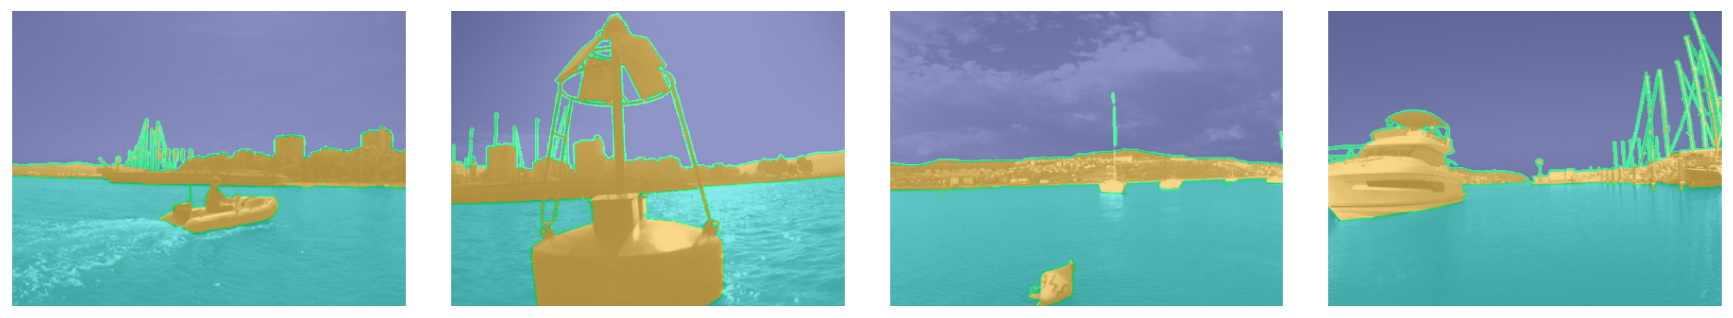
\includegraphics[width=\textwidth]{figures/MaSTr1325/official-annotation.jpg}
        \caption{}
        \label{fig:mastr1325}
    \end{subfigure}
    \hfill
    % MariShipSeg-HEU
    \centering
    \begin{minipage}{0.49\textwidth}
    \begin{subfigure}[b]{0.75\textwidth}
        \centering
        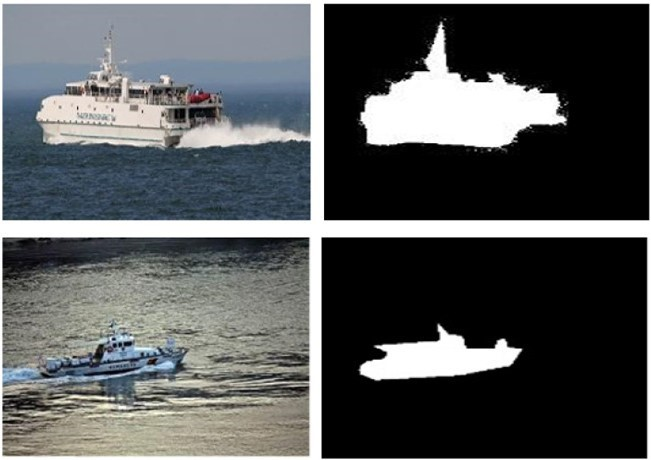
\includegraphics[width=\textwidth]{figures/D_MariShipSeg-HEU.jpg}
        \caption{}
        \label{fig:marishipseg}
    \end{subfigure}
    \hfill
    \end{minipage}
     % Foggy
     \hspace{-0.1\textwidth}
    \begin{minipage}{0.49\textwidth}
    \centering
    \begin{subfigure}[b]{1\textwidth}
        \centering
        \includegraphics[width=\textwidth]{figures/D_Foggy.jpg}
        \caption{}
        \label{fig:foggy}
    \end{subfigure}
    \hfill
    % Tampere
    \begin{subfigure}[b]{1\textwidth}
        \centering
        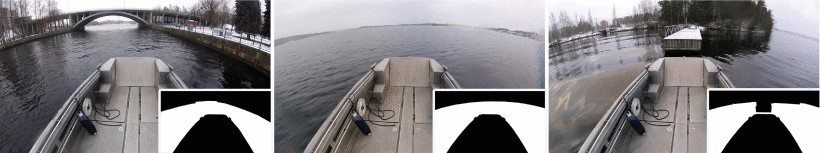
\includegraphics[width=\textwidth]{figures/D_tampere-waterseg.jpg}
        \caption{}
        \label{fig:tampere}
    \end{subfigure}
    \end{minipage}
    \hfill
    % OASIs
    \centering
    \begin{subfigure}[b]{0.9\textwidth}
        \centering
        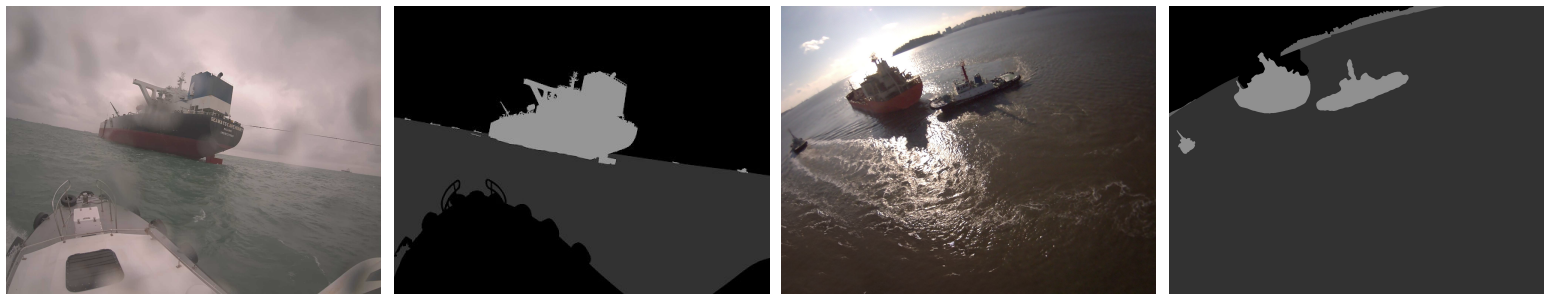
\includegraphics[width=\textwidth]{figures/OASIs/official-annotation.png}
        \caption{}
        \label{fig:oasis}
    \end{subfigure}
    \caption{The Annotation of different dataset: (a) MaSTr1325 \cite{MaSTr1325}, (b) MariShipSeg-HEU \cite{marishipseg},
    (c) Tampere Waterseg \cite{tampere}, (d) Foggy ShipInsseg \cite{foggy}, (e) OASIs \cite{OASIs}.}
    \label{fig:dataset-compare}
\end{figure}

Compared to datasets in the UGV domain, such as CamVid \cite{CamVid} and CityScapes \cite{Cityscapes} 
(as shown in Table \ref{tab:dataset-compare}), USV datasets are notably smaller in scale and have fewer annotation 
classes. This highlights the limited availability of marine datasets, which results in models trained on these 
datasets being less effective at handling unseen scenarios. USVs, however, are more likely to encounter novel 
environments due to factors such as varying weather conditions and camera instability from wave-induced motion. 
BDL, with its advanced inference capabilities, offers significant potential to address these challenges and enhance 
model robustness in unpredictable marine settings. In BDL methods, Kendall \cite{whatuncertaintydoweneed} employed 
the CamVid dataset to assess the effectiveness of Bayesian SegNet in uncertainty estimation. Additionally, Mukhoti 
and Gal \cite{evaluateBDL} investigated uncertainty evaluation metrics using the Cityscapes dataset. Despite these 
advancements, no models have yet been trained for marine semantic segmentation in USV domain. This paper proposes 
to harness BDL techniques to enhance the robustness of USV environmental perception by improving uncertainty 
estimation.

% table
\begin{table}[ht!]
    \centering
    \caption{Comparison of size and annotation richness between UGV and USV datasets.}
    \label{tab:dataset-compare}
    \begin{tabular}{c|c|c|c}
    \textbf{Dataset} & \textbf{Field} & \textbf{Number of Annotated Image } & \textbf{Number of Classes for Annotation} \\ \hline
    CamVid \cite{CamVid} & UGV & 701  & 32 \\ \hline
    CityScapes \cite{Cityscapes} & UGV & 5000  & 30 \\ \hline
    MaSTr1325 \cite{MaSTr1325} & USV & 1325  & 4 \\ \hline
    OASIs \cite{OASIs} & UGV & 445 & 4 \\ \hline
    \end{tabular}
\end{table}